% $Id: template.tex 11 2007-04-03 22:25:53Z jpeltier $

\documentclass{vgtc}                          % final (conference style)
%\documentclass[review]{vgtc}                 % review
%\documentclass[widereview]{vgtc}          % wide-spaced review
%\documentclass[preprint]{vgtc}               % preprint
%\documentclass[electronic]{vgtc}             % electronic version

%% Uncomment one of the lines above depending on where your paper is
%% in the conference process. ``review'' and ``widereview'' are for review
%% submission, ``preprint'' is for pre-publication, and the final version
%% doesn't use a specific qualifier. Further, ``electronic'' includes
%% hyperreferences for more convenient online viewing.

%% Please use one of the ``review'' options in combination with the
%% assigned online id (see below) ONLY if your paper uses a double blind
%% review process. Some conferences, like IEEE Vis and InfoVis, have NOT
%% in the past.

%% Figures should be in CMYK or Grey scale format, otherwise, colour 
%% shifting may occur during the printing process.

%% These three lines bring in essential packages: ``mathptmx'' for Type 1 
%% typefaces, ``graphicx'' for inclusion of EPS figures. and ``times''
%% for proper handling of the times font family.

\usepackage{mathptmx}
\usepackage{graphicx}
\usepackage{times}

%% We encourage the use of mathptmx for consistent usage of times font
%% throughout the proceedings. However, if you encounter conflicts
%% with other math-related packages, you may want to disable it.

%% If you are submitting a paper to a conference for review with a double
%% blind reviewing process, please replace the value ``0'' below with your
%% OnlineID. Otherwise, you may safely leave it at ``0''.
\onlineid{0}

%% declare the category of your paper, only shown in review mode
\vgtccategory{Research}

%% allow for this line if you want the electronic option to work properly
\vgtcinsertpkg

%% In preprint mode you may define your own headline.
%\preprinttext{To appear in an IEEE VGTC sponsored conference.}

%% Paper title.

\title{Preparing Ray Tracing for Exascale}

%% This is how authors are specified in the conference style

%% Author and Affiliation (single author).
%%\author{Roy G. Biv\thanks{e-mail: roy.g.biv@aol.com}}
%%\affiliation{\scriptsize Allied Widgets Research}

%% Author and Affiliation (multiple authors with single affiliations).
\author{
  Ellen A. Porter
  \thanks{e-mail: \texttt{ellen.porter@wsu.edu}} %
  \and
  Robert R. Lewis
  \thanks{e-mail: \texttt{bobl@tricity.wsu.edu}}}

\affiliation{
  \scriptsize Washington State University, Tri-Cities \\
  Program in Engineering and Computer Science}

%% Author and Affiliation (multiple authors with multiple affiliations)
%%\author{Roy G. Biv\thanks{e-mail: roy.g.biv@aol.com}\\ %
%%        \scriptsize Starbucks Research %
%%\and Ed Grimley\thanks{e-mail:ed.grimley@aol.com}\\ %
%%     \scriptsize Grimley Widgets, Inc. %
%%\and Martha Stewart\thanks{e-mail:martha.stewart@marthastewart.com}\\ %
%%     \parbox{1.4in}{\scriptsize \centering Martha Stewart Enterprises \\ Microsoft Research}}

%% A teaser figure can be included as follows, but is not recommended since
%% the space is now taken up by a full width abstract.
%\teaser{
%  \includegraphics[width=1.5in]{sample.eps}
%  \caption{Lookit! Lookit!}
%}

%% Abstract section.
\abstract{Ideas for titles: \\
Ray Tracing for Exascale Computing. \\
An approahc for Ray Tracing on Exascale Computers. \\
Adapting Ray Tracing for Exascale. \\

To reach exascale computing, significant hardware and software 
changes will be introduced to high-perfomance computing (HPC).  
Applications will need to adapt as the architecture of supercomputers 
change.  In this paper we explore the history of ray tracing given 
architecture changes and propose a methodology using the Intel 
Concurrent Collections (CnC) Programming Model and Intel Embree 
Ray Tracing Engine to build scalable ray tracing system. \\

And this is what references look like~\cite{ware:2004:IVP}.

} % end of abstract

%% ACM Computing Classification System (CCS). 
%% See <http://www.acm.org/class/1998/> for details.
%% The ``\CCScat'' command takes four arguments.

\CCScatlist{ 
  \CCScat{K.6.1}{Management of Computing and Information Systems}%
{Project and People Management}{Life Cycle};
  \CCScat{K.7.m}{The Computing Profession}{Miscellaneous}{Ethics}
}

%% Copyright space is enabled by default as required by guidelines.
%% It is disabled by the 'review' option or via the following command:
% \nocopyrightspace

%%%%%%%%%%%%%%%%%%%%%%%%%%%%%%%%%%%%%%%%%%%%%%%%%%%%%%%%%%%%%%%%
%%%%%%%%%%%%%%%%%%%%%% START OF THE PAPER %%%%%%%%%%%%%%%%%%%%%%
%%%%%%%%%%%%%%%%%%%%%%%%%%%%%%%%%%%%%%%%%%%%%%%%%%%%%%%%%%%%%%%%%

\begin{document}

%% The ``\maketitle'' command must be the first command after the
%% ``\begin{document}'' command. It prepares and prints the title block.

%% the only exception to this rule is the \firstsection command
\firstsection{Introduction}

\maketitle

%% \section{Introduction} 

Reaching exascale performance goals will require changes to node 
and system architecture. \\

Programming models and runtime systems are advancing as well to 
take advantage of the new systems. \\

Changes to the runtime: tuning hints \\
Changes to the models:  hierarchical programming models (CnC) \\

Current algorithms will need to be rewritten to take full advantage 
of the benifits of these new systems in order to scale to exascale. \\

Ray tracing algorithms have adapted in the past to hardware advances. \\

Some methods that did not work before due to load balancing may work well. \\

Summary of what we need in an application designed for future exascale systems 
and description of how our approach should work well.

Other features of exascale we can take advantage of (hierarchy?)

Future directions. \\

\section{Reaching Exascale}
Motivation: Moore's law
\subsection{Hardware Changes}
Heterogeneity, node failures
\subsection{Software Changes}
x86, MPI, OpenMP \\ 
Optimize for data movement, 
communication avoidance algorithms \\

\section{CnC Programming Model}
Model built for task based runtimes, work moves to data, 
relies on tag collections
\subsection{Tag Collections}
Used to organize steps and items
\subsection{Steps}
Computation to be done
\subsection{Item Collections}
Data to be used
\subsection{Tuning}
Hints that can be provided to the runtime \\

\section{Adapting Ray Tracing}
Modifications made for parallel ray tracing
\subsection{History/Previous Work?}
Discuss single node to distributed systems
\subsection{Changes for Future Systems}
Discuss reducing data movement and avoiding communication 

\begin{table}
  \caption{Vis Paper Acceptance Rate}
  \label{vis_accept}
  \scriptsize
  \begin{center}
    \begin{tabular}{cccc}
      Year & Submitted & Accepted & Accepted (\%)\\
    \hline
      1994 &  91 & 41 & 45.1\\
      1995 & 102 & 41 & 40.2\\
      1996 & 101 & 43 & 42.6\\
      1997 & 117 & 44 & 37.6\\
      1998 & 118 & 50 & 42.4\\
      1999 & 129 & 47 & 36.4\\
      2000 & 151 & 52 & 34.4\\
      2001 & 152 & 51 & 33.6\\
      2002 & 172 & 58 & 33.7\\
      2003 & 192 & 63 & 32.8\\
      2004 & 167 & 46 & 27.6\\
      2005 & 268 & 88 & 32.8\\
      2006 & 228 & 63 & 27.6
    \end{tabular}
  \end{center}
\end{table}

\section{Methodology}

\begin{figure*}[htb]
  \centering
  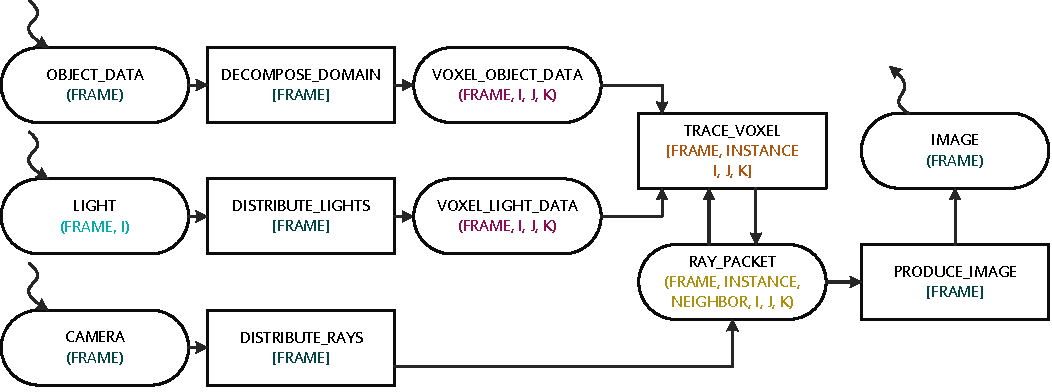
\includegraphics[width=\textwidth]{drawings/CnC.pdf}
  \caption{CnC graph}
\end{figure*}

High level description

\subsection{CnC Steps}
Details on the CnC Steps implemented (code?)

\subsubsection{Decompose Domain}
\subsubsection{Distribute Lights}

\begin{figure}[htb]
  \centering
  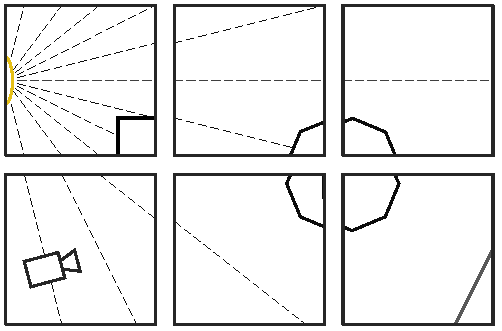
\includegraphics[width=\columnwidth]{drawings/Lights1.pdf}
  \caption{Light Source Rays}
\end{figure}

\begin{figure}[htb]
  \centering
  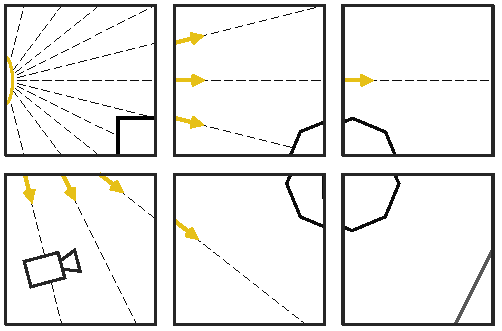
\includegraphics[width=\columnwidth]{drawings/Lights2.pdf}
  \caption{Distributed Point Source Rays}
\end{figure}

\subsubsection{Distribute Rays}

\begin{figure}[htb]
  \centering
  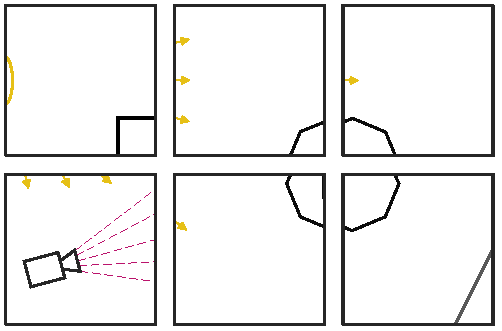
\includegraphics[width=\columnwidth]{drawings/Trace1.pdf}
  \caption{Distribute Rays}
\end{figure}

\subsubsection{Trace Voxel}
Embree kernel ray tracer

\begin{figure}[htb]
  \centering
  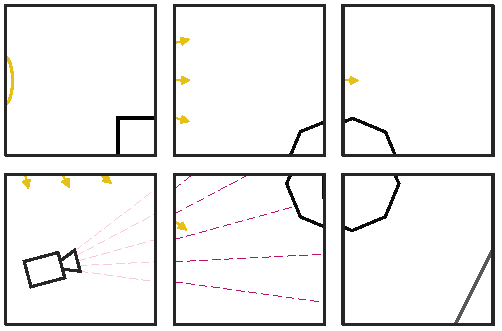
\includegraphics[width=\columnwidth]{drawings/Trace2.pdf}
  \caption{Trace Voxel}
\end{figure}

\begin{figure}[htb]
  \centering
  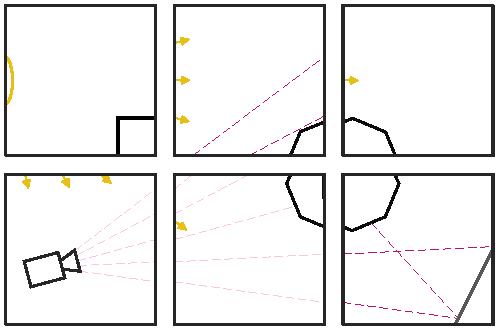
\includegraphics[width=\columnwidth]{drawings/Trace3.pdf}
  \caption{Trace Voxel}
\end{figure}

\begin{figure}[htb]
  \centering
  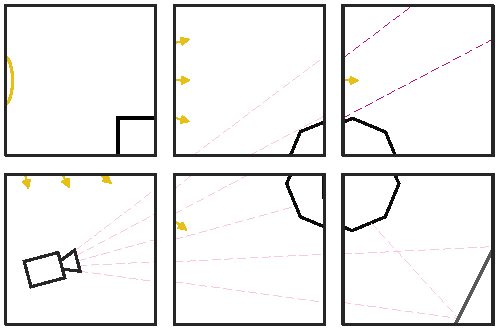
\includegraphics[width=\columnwidth]{drawings/Trace4.pdf}
  \caption{Trace Voxel}
\end{figure}

\subsubsection{Step: Produce Image}

\subsection{CnC Item Collections}
Details on the data (code?)

\subsubsection{Object Data}
\subsubsection{Voxel Object Data}
\subsubsection{Light}
\subsubsection{Voxel Light Data}
\subsubsection{Camera}
\subsubsection{Ray Packet}
\subsubsection{Image}

\subsection{Tuning Spec}
If we get to adding a tuning spec, describe and show code

\subsection{Running the application}
Do we need a section describing how to run the code?

\subsection{Performance}
System where we ran the code, results summary \\

\section{Other Exascale Features}
\subsection{Hierarchy}
Dynamic scenes, checkpoint and restart \\

\section{Future Directions}
Global illumination \footnote{Footnotes appear at the bottom of the column}. \\

\section{Conclusion}
Summary \\

%% if specified like this the section will be ommitted in review mode
\acknowledgements{
The authors wish to thank A, B, C.  CnC team at RICE? Intel for the cluster?}

\bibliographystyle{abbrv}
%%use following if all content of bibtex file should be shown
%\nocite{*}
\bibliography{template}
\end{document}
